%% ---------------------------------------------------------------------------
%% intro.tex
%%
%% Introduction
%%
%% $Id: intro.tex 1477 2010-07-28 21:34:43Z palvarado $
%% ---------------------------------------------------------------------------

\chapter{Introducción}
\label{chp:intro}

%En la \nt{introducción} deben quedar completamente claros los siguientes
%aspectos, cuyo significado depende del tipo concreto de tesis:
%
%\begin{compactitem}
%\item Contexto
%\item Problema
%\item Esbozo de solución
%\item Objetivos y estructura
%\end{compactitem}
%
%El contexto corresponde al entorno donde se desarrolla el proyecto de
%tesis, que puede ser el área general de aplicación, un dominio de
%problemas, etc. El problema concreto se sintetiza usualmente en una
%frase o pregunta. Esta pregunta debería ser una consecuencia a la que
%se llega después de realizar el desarrollo del contexto. Del
%planteamiento del problema se deriva cuál es el objetivo del trabajo
%en particular, que a su vez debe conducir al lector de forma natural
%al esbozo de la solución del problema a tratar en la
%tesis. Generalmente para aclarar la solución se hace uso de un
%diagrama de bloques o diagrama de flujo general, es decir, desde un
%nivel de abstracción alto, donde no sea necesario entrar en detalles
%técnicos. Usualmente este diagrama y su breve explicación dictan cuál
%debe ser la estructura del resto del tesis, que es mencionada siempre
%al final de la introducción.
%
%Una buena introducción debe lograr que el lector tenga interés de leer el resto
%del tesis.
%
%Es recomendable dividir la tesis en secciones, nombradas cada una de acuerdo a
%su contenido. \textbf{Jamás} utilice los nombres de la guía como
%``\emph{Problema existente e importancia de su solución}'', sino algo como ``La
%deforestación en Costa Rica'' o lo que se adecúe a su problema en particular.
%
%Recuerde que en español solo la primera letra del título va en mayúscula
%(exceptuando nombres propios, por supuesto).

El mejoramiento de las im\'agenes es un proceso en el que por medio de diferentes t\'ecnicas se obtiene un realce de las caracter\'isticas o informaci\'on relevante y la atenuaci\'on de informaci\'on poco importante o no deseada. Esto permite mejorar la efectividad de m\'etodos de segmentaci\'on, rastreo de objetos, clasificaci\'on y otras t\'ecnicas de reconocimiento de patrones y el aprendizaje autom\'atico. 


Los filtros espaciales son ampliamente utilizados para la reducci\'on de los diferentes tipos de ruido encontrados en las im\'agenes. Muchas veces se emplean en combinación con t\'ecnicas como la ecualizaci\'on de histogramas, que permite obtener una mejora en el contraste; o Unsharp Masking (USM) para resaltar los bordes.

Uno de los filtros con mejor resultado en la reducción de ruido es el Non-Local Means (NLM) propuesto en \textcite{1467423}, ya que se basa en la similitud entre los vecindarios de los pixeles contenidos en una ventana de búsqueda deslizante para el ponderamiento del peso asignado a cada pixel. Este enfoque ha demostrado muy buenos resultados con una menor p\'erdida de detalles (como por ejemplo los bordes) en comparaci\'on con otros filtros como el de mediana y el bilateral \cite{calderon2016first}. Es importante resaltar que este algoritmo es altamente paralelizable, debido a que no existe dependencia en el c\'alculo de los pixeles que componen la imagen. 

Existen mejoras desarrolladas a partir del algoritmo NLM, un enfoque novedoso es el propuesto en \textcite{7160148} llamado Deceived Non-Local Means (DNLM). Presenta una combinaci\'on del m\'etodo Unsharp Masking (USM) con el filtro NLM por medio del desacoplamiento de la imagen utilizada en el pesado y la imagen usada en el filtrado. Esto permite reducir los artefactos no deseados en las im\'agenes (efecto de anillo) generados por el enfoque convencional, es decir, al aplicar primero el m\'etodo USM y posteriormente el filtro NLM.  

Uno de los principales inconvenientes del filtro NLM es su complejidad computacional: En el peor de los casos, para una imagen de entrada de $N$ pixeles utilizando un tamaño de ventana deslizante de $A\times B = N$ y un tamaño de vecindario de $A\times B = N$, la complejidad computacional es de $\mathcal{O}(N^{3})$. 

Lo anterior provoca que el tiempo de procesamiento del filtro NLM sea una limitante importante a considerar, en especial si se planea utilizar para una tarea en tiempo real o en el preprocesado de grandes vol\'umenes de im\'agenes (en el caso de sets de datos para aprendizaje autom\'atico). 

Una forma de reducir la complejidad computacional del filtro es mediante el uso de optimizaciones o aproximaciones del algoritmo. Este proyecto pretende continuar el trabajo realizado previamente, que consisti\'o en el desarrollo de una propuesta de optimizaci\'on para el filtro DNLM por medio del uso de Im\'agenes Integrales y la Transformada R\'apida de Fourier (DNLM-IIFFT). Esta optimizaci\'on permite reducir la complejidad del algoritmo a  $\mathcal{O}(N^{2}\log(N))$. Los resultados experimentales arrojan una aceleraci\'on de hasta 10 veces en el procesamiento de una imagen de 720p. Si bien estos resultados presentan una aceleraci\'on importante, se deben explorar t\'ecnicas de paralelizaci\'on que permitan reducir a\'un m\'as el tiempo de ejecuci\'on del algoritmo. 

\begin{figure}[htb]
  \centering
  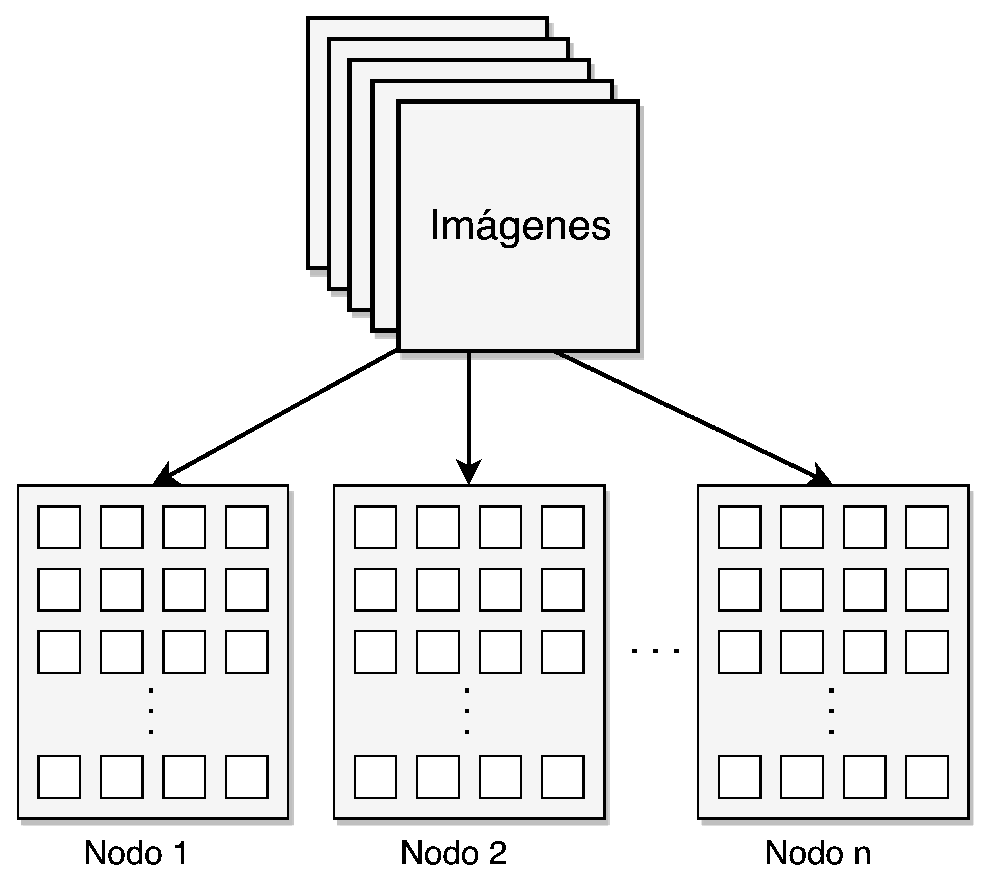
\includegraphics[width=0.9\textwidth]{blockD}
  \caption{Diagrama de bloques de la soluci\'on}
  \label{fig:ltxfig}
\end{figure}

*COMENTAR Y HACER REFERENCIA SOBRE FIGURA*

\section{Objetivos y estructura del documento}

\index{objetivos}

Este trabajo tiene como objetivo la paralelizaci\'on del filtro DNLM-IIFFT optimizado para la arquitectura Xeon Phi Knights Landing, que permita el procesamiento eficiente de grandes vol\'umenes de im\'agenes.
En este trabajo se realiza una implementaci\'on paralela del filtro DNLM-IFFT (modificaci\'on del filtro NLM) en sistemas multi-nodo optimizados para la arquitectura Intel Knights Landing, con la finalidad de realizar procesamiento concurrente y de alto rendimiento de grandes conjuntos de im\'agenes. 



%Esta plantilla LaTeX tiene como objetivo simplificar la construcción del
%documento de tesis, presentando ejemplo de figuras y tablas, así como otorgar
%una plataforma de compilación en GNU/Linux que simplifique la administración de
%todo el documento.
%
%La última sección de la introducción usualmente sí tiene un título estandar que
%es ``Objetivos y estructura del documento'', donde se presentan \emph{en prosa}
%los objetivos general y específicos que ha tenido el proyecto de tesis,
%así como la estructura de la tesis (por ejemplo, ``en el siguiente capítulo se
%esbozan los fundamentos teóricos necesarios para explicar en el
%capítulo~\ref{ch:solucion} la propuesta realizada$\ldots$''

%%% Local Variables: 
%%% mode: latex
%%% TeX-master: "main"
%%% End: 
